\chapter{影響中風的因素}
\section{Analysis of Contingency Table}
\subsection{中風與性別}
\begin{itemize}
    \item 基本假設:性別與中風沒有關聯
\end{itemize}
\begin{center}
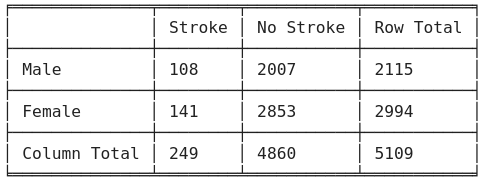
\includegraphics[width=8cm]{./two_by_two_table/gender_stroke.png}
\end{center}
\begin{itemize}
    \item 註記: 有一個性別是Other,被拿掉了
    \item Odds ratio $\hat{\theta}=1.089$
    \item 95\% Confidence Interval of $\log{(\hat{\theta})}=(-0.172, 0.342)$
    \item 結論:中風跟性別是獨立的,符合我們一開始的猜想
\end{itemize}

\subsection{中風與居住環境}
\begin{itemize}
    \item 基本假設:只有一點點關聯,鄉下的中風比例可能比住在城市的低
\end{itemize}
\begin{center}
    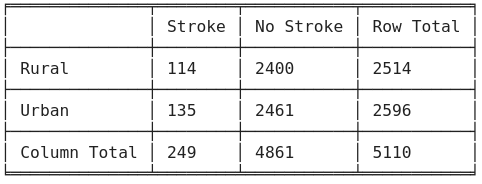
\includegraphics[width=8cm]{./two_by_two_table/resitype_stroke.png}
\end{center}
\begin{itemize}
    \item Odds ratio $\hat{\theta}=0.866$
    \item 95\% Confidence Interval of $\log{(\hat{\theta})}=(-0.400, 0.112)$
    \item 雖然資料符合我們的猜想,鄉下中風的比例比較低,但是95\%的信賴區間包含0,表示 $\log{(\hat{\theta})}$ 與0無顯著差異
    \item 結論:中風與居住環境是獨立的
\end{itemize}

\subsection{中風與婚姻}
\begin{itemize}
    \item 基本假設:婚姻與中風沒有關聯
\end{itemize}
\begin{center}
    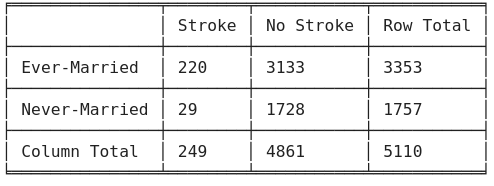
\includegraphics[width=8cm]{./two_by_two_table/evermarry_stroke.png}
\end{center}
\begin{itemize}
    \item Odds ratio $\hat{\theta}=4.184$
    \item 95\% Confidence Interval of $\log{(\hat{\theta})}=(1.040, 1.823)$
    \item 95\%的信賴區間不包含0,表示 $\log{(\hat{\theta})}$ 與0有顯著差異。
    \item 結論:跟我們的基本假設相反,中風跟"有無結過婚"有關聯
\end{itemize}
Fix column比較:
\begin{itemize}
    \item 中風患者: $\frac{\text{Ever-Married}}{\text{Never-Married}}=7.59$
    \item 非中風者: $\frac{\text{Ever-Married}}{\text{Never-Married}}=1.81$
    \item 中風患者中"結婚與沒結婚"的比例高於非中風者
\end{itemize}

\subsection{中風與壓力}
\begin{itemize}
    \item 基本假設:壓力愈大的人愈容易中風
\end{itemize}
\begin{center}
    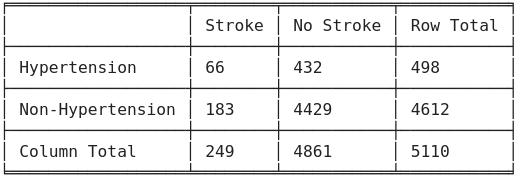
\includegraphics[width=8cm]{./two_by_two_table/hypert_stroke.png}
\end{center}
\begin{itemize}
    \item Odds ratio $\hat{\theta}=3.698$
    \item 95\% Confidence Interval of $\log{(\hat{\theta})}=(1.009, 1.606)$
    \item 95\%的信賴區間不包含0,表示 $\log{(\hat{\theta})}$ 與0有顯著差異。
    \item 結論:中風跟壓力有關聯
\end{itemize}
Fix column比較:
\begin{itemize}
    \item 中風患者: $\frac{\text{Hypertension}}{\text{Non-Hypertension}}=0.36$
    \item 非中風者: $\frac{\text{Hypertension}}{\text{Non-Hypertension}}=0.10$
    \item 符和基本假設,壓力愈大的人愈容易中風
\end{itemize}

\subsection{中風與心臟病}
\begin{itemize}
    \item 基本假設:中風是心血管疾病,要與心臟病相關
\end{itemize}
\begin{center}
    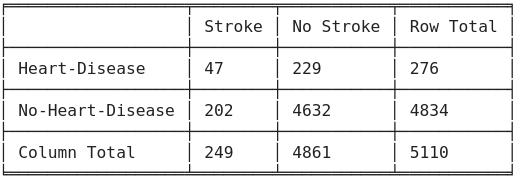
\includegraphics[width=8cm]{./two_by_two_table/heartd_stroke.png}
\end{center}
\begin{itemize}
    \item Odds ratio $\hat{\theta}=4.706$
    \item 95\% Confidence Interval of $\log{(\hat{\theta})}=(1.205, 1.893)$
    \item 95\%的信賴區間不包含0,表示 $\log{(\hat{\theta})}$ 與0有顯著差異。
    \item 結論:中風跟心臟病有關聯
\end{itemize}
Fix column比較:
\begin{itemize}
    \item 中風患者: $\frac{\text{Heart-Disease }}{\text{No-Heart-Disease}}=0.23$
    \item 非中風者: $\frac{\text{Heart-Disease }}{\text{No-Heart-Disease}}=0.05$
    \item 符和基本假設,中風患者中有心臟病的比例高
\end{itemize}

\subsection{中風與抽煙習慣}
\begin{itemize}
    \item 基本假設:有抽煙的人比較容易中風
\end{itemize}
\begin{center}
    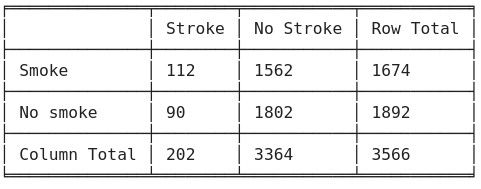
\includegraphics[width=8cm]{./two_by_two_table/smoke_stroke.png}
\end{center}
\begin{itemize}
    \item 註記: unknown有1544個資料點,被拿掉了
    \item 註記: smoke包含smokes與formerly smoked
    \item Odds ratio $\hat{\theta}=1.436$
    \item 95\% Confidence Interval of $\log{(\hat{\theta})}=(0.076, 0.647)$
    \item 95\%的信賴區間不包含0,表示 $\log{(\hat{\theta})}$ 與0有顯著差異。
    \item 結論:中風跟抽煙有關聯。但相比於婚姻、壓力與心臟病,抽煙的$\hat{\theta}$比較靠近$1$,表示抽煙相對來說不是一個重要的因子
\end{itemize}
Fix column比較:
\begin{itemize}
    \item 中風患者: $\frac{\text{Smoke}}{\text{No smoke}}=1.24$
    \item 非中風者: $\frac{\text{Smoke}}{\text{No smoke}}=0.87$
    \item 符和基本假設,中風患者中有抽煙的比例高
\end{itemize}

\subsection{中風與年齡}
\begin{center}
    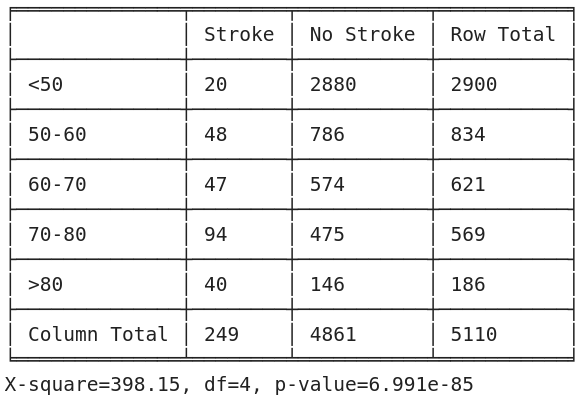
\includegraphics[width=8cm]{./chisquare/age_stroke.png}
\end{center}

\subsection{中風與血糖}
分類依據:
\begin{center}
    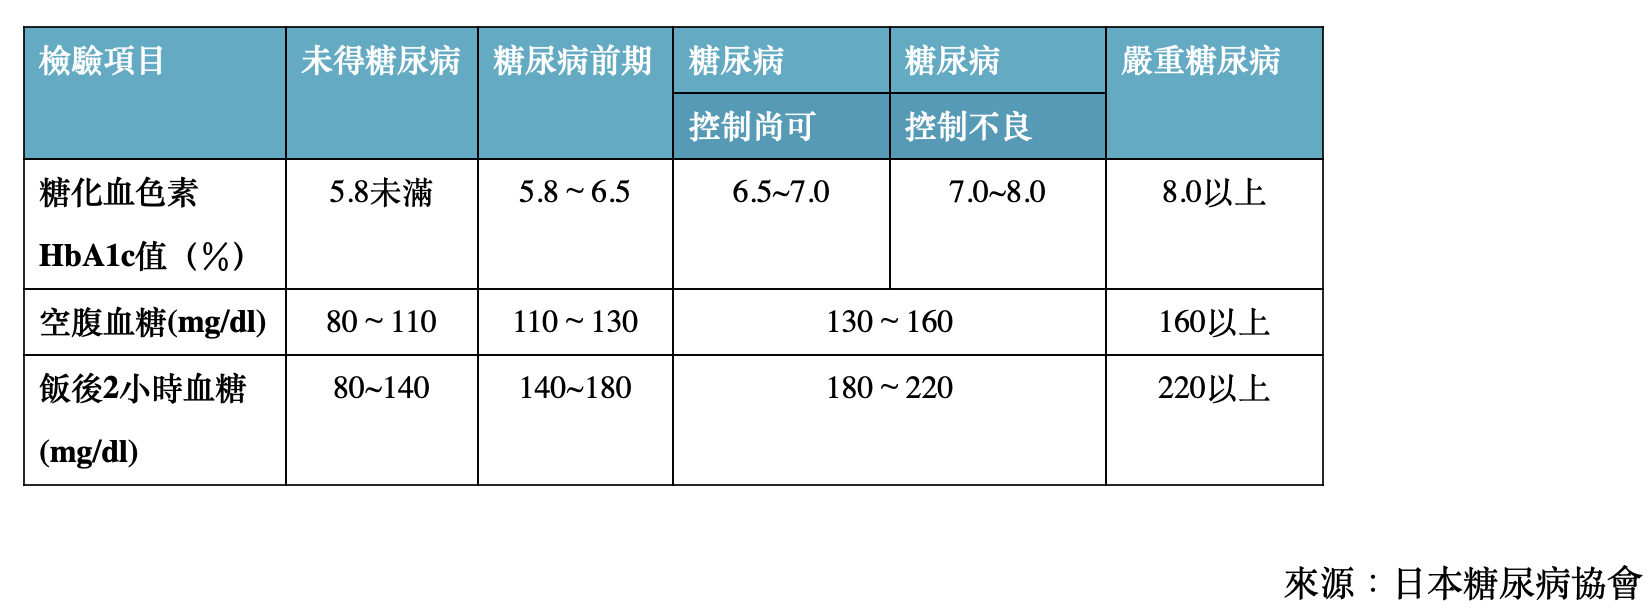
\includegraphics[width=8cm]{./images/glucose_category_ref.png}
\end{center}
$\chi^2$ test:
\begin{center}
    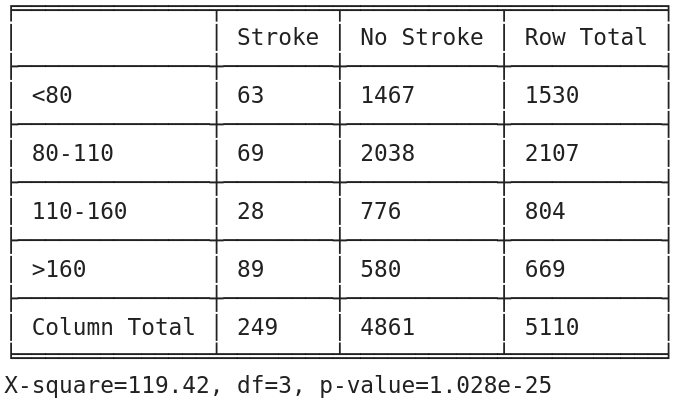
\includegraphics[width=8cm]{./chisquare/glucose_stroke.png}
\end{center}

\subsection{中風與BMI}
分類依據:
\begin{center}
    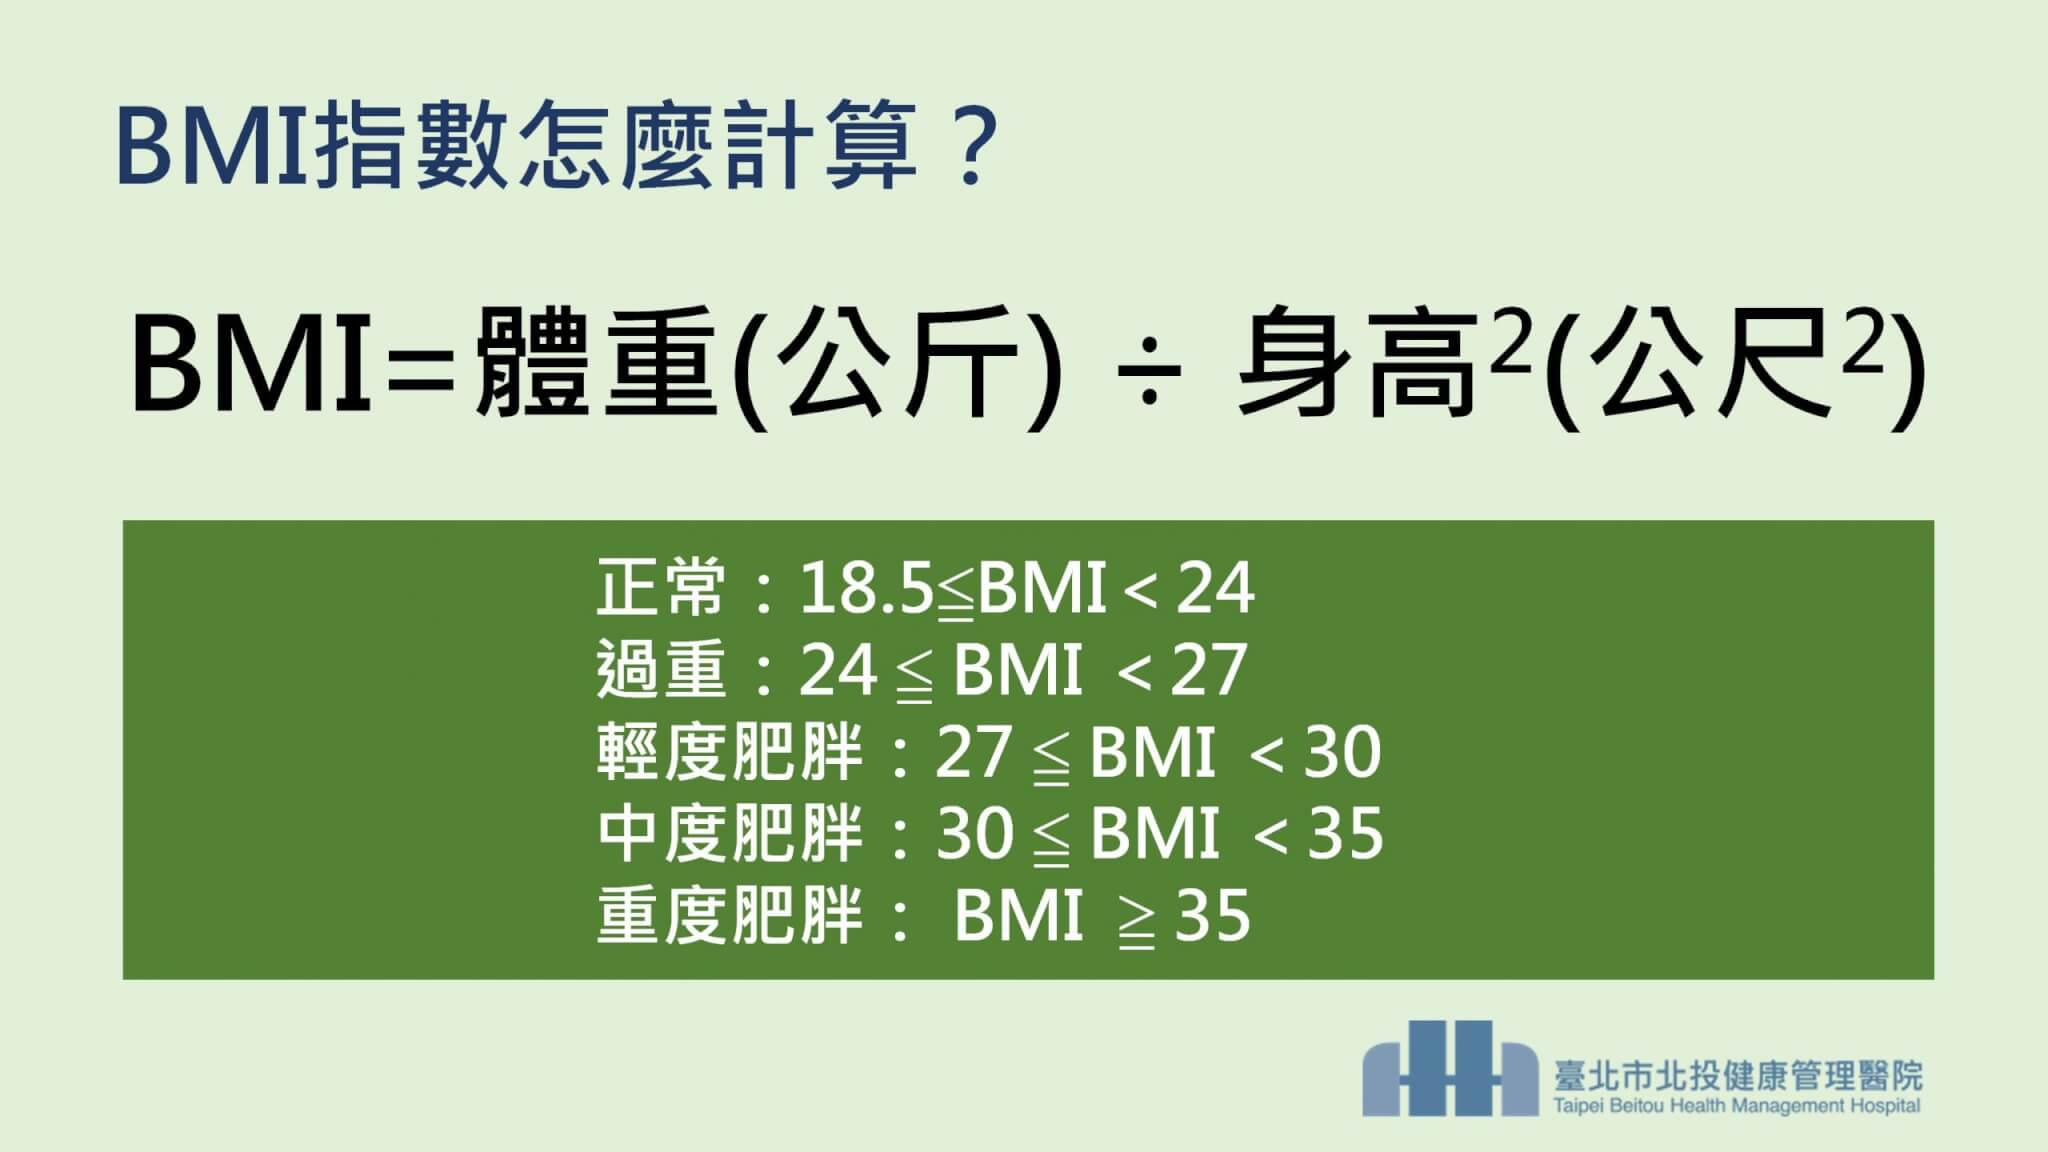
\includegraphics[width=8cm]{./images/bmi_category_ref.jpg}
\end{center}
$\chi^2$ test:
\begin{center}
    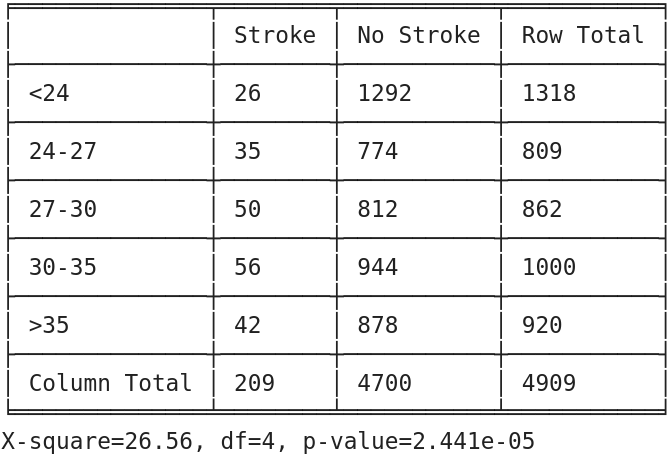
\includegraphics[width=8cm]{./chisquare/bmi_stroke.png}
\end{center}

